\chapter{Asking Dallas Billionaires How They Got Rich!}

This chapter follows Lecture 5 of the \emph{Hard Knocks Interviews} series from School of Hard Knocks, curated by LazyingArt LLC. The lecture does not begin as an argument on a board. It begins as a hunt. A passerby points toward a billionaire, the host changes direction in real time, and the governing question arrives before any framework has been announced: how did you get rich? What follows is therefore best read as a sequence of field observations gradually tightened into rules. We will keep that order. We will preserve the lecture's movement from encounter to claim, from claim to mechanism, and from mechanism to a more durable philosophy of wealth, risk, and commercial judgment.

\section{Street Encounters as Method}

Before the lecture settles into its main body, it gives us a quick preview of scale. We hear, almost in montage form, of a little over \(\$40\) million in a year, about \(\$200\) million personal in a year, a company doing about \(\$1.5\) billion in volume, and many billions from the sale of 7-Eleven. The effect is not accidental. The lecture wants the magnitude in place before it explains the path.

Only then does the host slow down and tell us where we are. Highland Park is presented as one of the richest municipalities in the United States: no state income tax, old money, new money, and some of the highest household incomes in the country. The neighborhood is not merely scenery. It is the lecture's chosen laboratory. The host has come here, he says, to figure out how people built their wealth and what it actually takes to become financially free.

The method matters as much as the content. A Ferrari, a lobby, a passing introduction, and a brief exchange are not treated as noise. They are treated as live probes. The lecture teaches us first how to ask, and only afterward what kind of answer might count. Very early, one thesis begins to recur: serious wealth, in this interview world, is repeatedly tied to ownership. We should record that as speaker doctrine rather than established law, but the whole lecture will keep returning to it.

\section{Building an Irresistible Company}

The first extended conversation is with Vic Keller, and here the lecture finds its first real backbone. Keller says he founded \(17\) companies and sold \(9\) of them. Later, in the host's recap, this is sharpened further: three of those sales were to Berkshire Hathaway. Whether or not we pause over that detail, the structural point is clear. We are no longer with someone describing a single lucky exit. We are listening to someone who has repeated the cycle enough times to speak in design principles.

The host asks the natural question: if selling a business is the dream, what is the best advice? Keller answers with two linked instructions. Build a company that is ``absolutely irresistible,'' with the best value proposition in the space, and hire the smartest, best people available, then help them get rich. The lecture is already doing something characteristic here: it refuses to separate product logic from people logic. The company becomes desirable to buyers not simply because it sells something useful, but because it concentrates value, capability, and incentive alignment in one place.

If we compress the speaker's business logic into a single schematic line, we may write
\begin{equation}
\text{Scale} \sim \text{focus} \times \text{talent quality} \times \text{time invested}.
\end{equation}
This is not a measured law from the lecture. It is a disciplined shorthand. Keller's point is that enterprise value is amplified when focus, people, and duration reinforce one another rather than pulling apart.

The lecture then makes its first surprising turn. Asked what industry he would enter if he had to start over, Keller does not name software, media, or some fashionable frontier. He says: car washes. He claims to be building hundreds of them, calls them the best business, and describes them as a kind of legal ATM machine. The host's surprise is pedagogically useful. A business thesis need not sound glamorous in order to be powerful. On the contrary, the lecture suggests that durable and repeatable demand may matter more than prestige.

\begin{remark}
The claims that car washes are ``recession-proof'' and ``depression-proof'' should be kept as the speaker's own emphatic doctrine. The lecture does not offer the economic evidence needed to elevate those phrases into proven general law.
\end{remark}

From there Keller returns to the people question and drives it harder. Asked what the secret to very large scale is, he does not talk about clever financial engineering. He says to spend one's time getting the best talent possible, investing in that talent deeply, and helping those people get to where you are. He then sharpens the thought with a memorable asymmetry: billionaires make millionaires, millionaires make billionaires, but he has never seen a billionaire make another billionaire. The line is not meant as a formal theorem. It is meant to suggest that scale is social. Wealth-building, at least in this lecture, is not merely accumulation. It is multiplication through other people's rise.

\subsection{Question \& Answer}

\paragraph{Question.} Should one diversify early, or should one concentrate?

\paragraph{Answer.} The lecture raises this tension explicitly and resolves it in favor of concentration, though not without acknowledging the appeal of safety. Diversification may be ``awesome,'' Keller says, but the people he knows who made the most money were laser-focused. They compounded growth ``every hour, every minute, every day, forever,'' became the best in the world at one thing, and only then earned the right to do many other things. The operative word is mastery. In the logic of this lecture, diversification belongs to protection; concentration belongs to magnitude.

The Keller section closes by widening from business method to personal philosophy. A line from an early partner is preserved: ``rich is loud and wealth is quiet.'' Then faith enters openly. Keller says he loves Jesus, that none of what he has is possible without Christ, and that health, money, and friends can all be lost while that relationship remains. The lecture does not try to neutralize this worldview. It leaves it where Keller puts it: inside the explanation of how he understands success itself.

\section{Cycles, First Deals, and Reverse Engineering}

The next major conversation returns us to the Ferrari owner from the opening. This is a useful structural move. What first appeared as a quick cold-open exchange is now expanded into a fuller line of thought. The host repeats the basic question, and the speaker answers with a blunt doctrine: yes, you have to be a business owner. His main business, he says, has most recently been oil and gas, with real estate besides, and he has been a business owner for \(35\) years.

This interview is the lecture's clearest stretch of practical commercial reasoning. The speaker explains that he once watched \emph{The Prize} and concluded that oil and gas is a boom-bust business. In boom times, people think the boom will never end. In busts, people think the industry will never return. He decided that the next time it busted, he would buy, and when the boom returned he would remember that it would not last forever. What matters here is not the industry label by itself. It is the structure of the thought.

\begin{definition}
The \emph{boom-bust heuristic} in this lecture is the rule of acting in one phase while preserving memory of the opposite phase. One buys in the bust while remembering the boom, and one restrains oneself in the boom while remembering the bust.
\end{definition}

\begin{figure}
\begin{center}
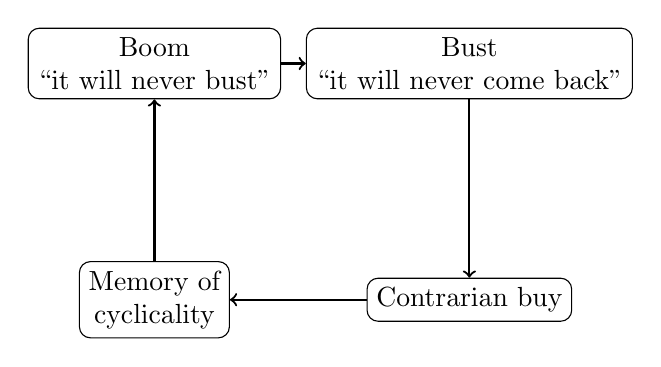
\begin{tikzpicture}[scale=1]
\node[draw, rounded corners, align=center] (boom) at (0,2) {Boom\\``it will never bust''};
\node[draw, rounded corners, align=center] (bust) at (4,2) {Bust\\``it will never come back''};
\node[draw, rounded corners, align=center] (buy) at (4,-1) {Contrarian buy};
\node[draw, rounded corners, align=center] (memory) at (0,-1) {Memory of\\cyclicality};
\draw[->, thick] (boom) -- (bust);
\draw[->, thick] (bust) -- (buy);
\draw[->, thick] (buy) -- (memory);
\draw[->, thick] (memory) -- (boom);
\end{tikzpicture}
\end{center}
\end{figure}

The speaker then reports a concrete scale:
\begin{equation}
R_{\text{oil+gas}} \approx \$40\times 10^6 \quad \text{in one year}.
\end{equation}
But the lecture immediately refuses to leave the number floating. The speaker says he came from no money, lived in a house heated by a wood stove, and worked in a lunchroom for free meals as a child. The number is there to mark outcome; the surrounding biography is there to restore motivational pressure.

\paragraph{Worked example.} The lecture becomes most mathematically explicit when the speaker describes his first distressed-loan purchase. He says he maxed out a credit card at \(\$70{,}000\), bought a package of failed loans with face value \(\$1.6\) million, and paid \(\$64{,}000\) for it. If we write
\[
F=\$1.6\times 10^6,
\qquad
P=\$64{,}000,
\]
then the paid fraction of face is
\begin{align}
d &= \frac{P}{F}
   = \frac{64{,}000}{1.6\times 10^6}
   = 0.04,\\
\delta &= 1-d = 0.96.
\end{align}
So the package was purchased at about \(4\%\) of face, or at about a \(96\%\) discount. The lecture is careful, however, not to let arithmetic masquerade as courage. The speaker says he felt terrible after doing it, called a friend about eleven years older than himself, and was told that the first deal is the hardest and will never feel that bad again. The number reveals the bargain. The story reveals the cost of acting before certainty arrives.

The interview then broadens. Asked what industry people should enter, the speaker answers: something where they have an edge. If everyone already thinks it is a great idea, then the opportunity has largely been priced in. Again the lecture is anti-consensus, or at least anti-late-consensus. A good idea is not only something true; it is something not yet fully absorbed by price and crowd behavior.

The host pushes outward once more: who doubted you, what role did your wife play, what does it mean to be rich, and is everyone built for entrepreneurship? The speaker's answers remain consistent. His wife believed in him when others did not. Money is part of a good life, but not the whole of it. Not everyone is built for entrepreneurship. The key discriminator, he says, is the ability to live with uncertainty and to trust oneself through dry times. The lecture is again binding business method to temperament.

\subsection{Question \& Answer}

\paragraph{Question.} How should we plan a life when uncertainty is inescapable?

\paragraph{Answer.} The lecture answers not by denying uncertainty, but by reversing the direction of thought. We are told to picture where we want to be in \(30\) years, not in exhaustive detail but in general form, and then to work backward. In compact notation we may write
\begin{equation}
A_0 = \mathcal{R}(T_{30}),
\end{equation}
where \(T_{30}\) is the long-horizon target state, \(A_0\) is present action, and \(\mathcal{R}\) denotes reverse engineering. This notation is a cautious reconstruction, but it preserves the lecture's logic.

\begin{figure}
\begin{center}
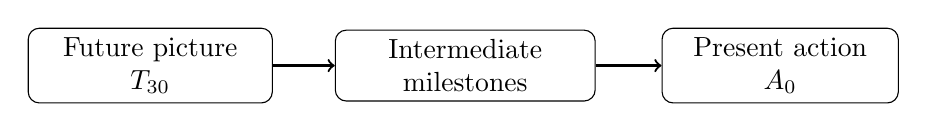
\begin{tikzpicture}[scale=1]
\node[draw, rounded corners, minimum width=3.1cm, align=center] (future) at (0,0) {Future picture\\\(T_{30}\)};
\node[draw, rounded corners, minimum width=3.3cm, align=center] (mid) at (4,0) {Intermediate\\milestones};
\node[draw, rounded corners, minimum width=3.0cm, align=center] (present) at (8,0) {Present action\\\(A_0\)};
\draw[->, thick] (future) -- (mid);
\draw[->, thick] (mid) -- (present);
\end{tikzpicture}
\end{center}
\end{figure}

The lecture's planning rule may therefore be read in three steps:
\begin{enumerate}
\item Form a broad picture of the desired future state \(T_{30}\).
\item Infer the milestones that would have to exist if that picture were ever to become real.
\item Choose present action \(A_0\) so that those milestones become reachable.
\end{enumerate}

The speaker compares this to taking a test when one already knows what will be on it. Preparation becomes more obvious. The lecture's point is not prediction. It is deliberateness.

\section{Recovery, Character, and Hiring Weakness}

At this stage the lecture deliberately jolts its social register. The next interview begins not with a large public company or a cyclical asset class, but with a federal penitentiary. The host says he first saw the man on a phone inside one. That shock is not incidental. The lecture is widening its account of where business competence can come from and what sort of human reconstruction may precede it.

The interviewee says he spent almost four years in prison. He also says that his family has an HVAC company, \(42\) years old, that began in the Tulsa area and was brought into Texas about a year and a half earlier. He reports a \(49\%\) exit about six months before the interview, says the deal came in at \(7\times\) what they had it for, places Oklahoma revenue at about \(\$3.5\) million, and hears the host summarize the outcome as roughly \(\$20\) million made on the transaction.

\begin{remark}
The numerical structure of this segment is incomplete. We preserve the reported \(49\%\) exit, \(7\times\) multiple, \(\$3.5\) million revenue, and host-side \(\$20\) million estimate, but the lecture does not supply enough detail to reconstruct a full valuation model.
\end{remark}

The speaker's own account of recovery is explicitly religious. Asked what brought him out of rock bottom and enabled him to help build a multi-million-dollar business, he answers: his relationship with Jesus Christ. Here again the lecture keeps faith inside the causal structure rather than relegating it to decorative testimony.

But the commercial mechanism is distinct and sharply stated. A former cellmate, an executive from Procter \& Gamble, told him to hire his weakness. That line deserves to be preserved with care because it condenses a management rule the lecture has been approaching from several angles. Strength is where one makes money, he says; weakness is where one keeps it. The formulation is not literally algebraic, but it has an operational form. If the enterprise is built only around what the founder does well, then blind spots become the leak through which value escapes. The correction is organizational rather than introspective: bring in people who are better than you exactly where you are fragile.

The prison narrative adds a second lesson about people. When nobody has anything, the speaker says, then one discovers what people really are, because there is little left to exchange except handshake, love, and loyalty. In the lecture's overall architecture this matters because it keeps character from becoming an abstract moral category. Character is shown here under deprivation, and then carried back into business as a practical condition of trust.

The section closes on a line of hope rather than method. The comeback, he says, can be greater than the setback. The lecture lets that line stand not as a proof, but as the emotional counterweight to the sections on uncertainty and sacrifice.

\section{Corporate Entrepreneurship and the Three-Part Survival Rule}

The lecture briefly breaks for promotion, then returns at a much larger institutional scale. This interruption is worth noting because it resets tempo: we move from prison and HVAC into Fortune 500 leadership. Jim Keyes arrives not merely as a wealthy individual but as a figure attached to 7-Eleven and Blockbuster. Before the host even reaches the main questions, Keyes says something that foreshadows the rest of the section: it is more important to teach people how to handle bad times than good times.

Only after that frame is established does the host ask about money. Keyes answers by distinguishing a single day from a single year and says that on the day he sold 7-Eleven the figure was many billions of dollars. He then locates that outcome against a childhood in a house with no running water. Again the lecture pairs extreme scale with severe scarcity, but here it does so to set up a different argument.

Asked what the most successful CEOs have in common, Keyes answers: fearlessness. He means the ability to transact without paralysis. Asked about relationships, he says they are everything, and that the most valuable resource of any company is the human resource. The lecture is now reaffirming, at corporate scale, a principle that earlier interviews stated at founder scale.

\begin{definition}
A \emph{corporate entrepreneur}, in the language of this lecture, is someone who behaves entrepreneurially inside a large structure: not sheltered from initiative, but given a more organized environment in which initiative can operate.
\end{definition}

This is Keyes's answer to the recurring question of whether everyone should simply become a founder. Not everybody is an entrepreneur in the same sense, he says, but that does not mean value-creating initiative disappears inside institutions. The corporate world may provide more structure while still rewarding entrepreneurial conduct.

\subsection{Question \& Answer}

\paragraph{Question.} Can one get rich without being a pure entrepreneur in the founder sense?

\paragraph{Answer.} The lecture answers yes, but with an important caveat. Structure is not a substitute for entrepreneurial behavior. The corporation may provide scaffolding, but one still has to act, initiate, and execute as though one were responsible for value rather than merely employed by it.

The strongest formal compression in the lecture appears when Keyes gives what is essentially a survival rule for business.

\begin{proposition}
Business survival, in Keyes's formulation, rests on three coupled terms:
\begin{equation}
\{\text{cash},\ \text{communications},\ \text{character}\}.
\end{equation}
Cash is the firm's oxygen, communications align the team, and character determines whether the firm survives when pressure arrives.
\end{proposition}

\begin{figure}
\begin{center}
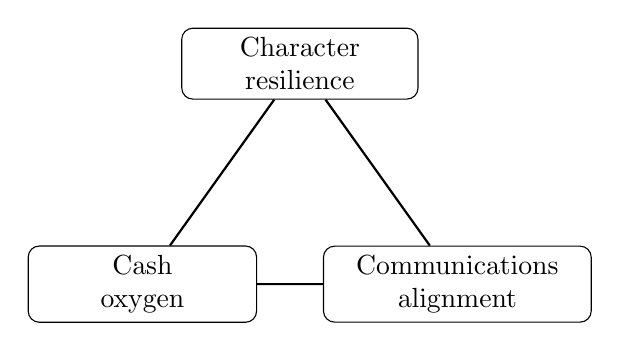
\begin{tikzpicture}[scale=1]
\node[draw, rounded corners, minimum width=2.9cm, align=center] (cash) at (0,0) {Cash\\oxygen};
\node[draw, rounded corners, minimum width=3.4cm, align=center] (comm) at (4,0) {Communications\\alignment};
\node[draw, rounded corners, minimum width=3.0cm, align=center] (char) at (2,2.8) {Character\\resilience};
\draw[thick] (cash) -- (comm) -- (char) -- (cash);
\end{tikzpicture}
\end{center}
\end{figure}

The lecture unpacks the triad in precisely that order. Cash flow must be watched through debt, payables, and receivables because firms can suffocate before their strategy has time to mature. Communications matter because frightened teams cannot execute. Character matters because trouble tests values, resilience, and self-confidence all at once. This is the lecture's nearest equivalent to a theorem, and it earns that status because it is not merely asserted; it is motivated by the prior movement through bad times, uncertainty, and people.

The section ends with an unexpected but revealing book recommendation. Keyes names the \emph{Boy Scout Handbook}. He then recites the Scout virtues. The lecture's point is not nostalgia. It is that leadership, at very large scale, may still depend on a moral vocabulary simple enough to be remembered and lived.

\section{Time, Culture, Sacrifice, and Choosing a Life}

The final major pivot was promised much earlier: later in the video, the host had said, a billionaire would let us tour his private jet. When the lecture finally arrives there, it does something disciplined with the spectacle. It allows the jet to create momentum, then immediately converts the spectacle into a problem about time.

Ben Pogue says his last commercial flight was in \(2018\), that he has had several planes since, and that he now flies about
\begin{equation}
H_{\text{flight}} \approx 300 \text{ hours}.
\end{equation}
Asked whether flying private makes one more money, he resists the easy answer. He calls it a luxury item. One simply has to accept what it costs. But then he gives the lecture's actual justification: time is the most precious commodity, and in that sense the plane is a time machine. The claim is not that private flying magically generates profit. The claim is narrower and more serious. Money can sometimes be exchanged for time recovered.

The tour itself reinforces a different motif: attention to detail. Soft panels, matte wood, a custom exterior, and the language of a car enthusiast all prepare the next business question, because they display a mind that treats objects as finished systems rather than as generic commodities. When the host asks how much the jet cost, Pogue says a new one would be around \(\$50\) million, that he put about \(\$5\) million into interior and paint, and that he paid probably about \(\$20\) million all in.

\begin{remark}
As earlier, the figures in this segment should be retained as reported claims rather than stitched into an exact accounting identity. The transcript is conversational, and one phrase in the cost explanation is clearly unstable.
\end{remark}

Only after the tour does the lecture name the business behind the wealth. Pogue says his main company was a second-generation construction firm, originally his father's company, taken over in \(2009\) and bought outright in \(2016\). Asked how he stood out in a crowded field, he gives an answer that now sounds familiar but appears in a distinct register: people and culture. Every company, he says, is in the people business and the service business whether it knows it or not.

This section pushes the people theme further than any earlier one. Relationships are not only important; people need to know that you care for them, that you will be there for them, and that high expectations do not cancel support. If they know that, he says, they will run through walls for you. What earlier speakers called talent and alignment, this speaker now describes as care joined to demanding standards.

The host then asks for the most life-changing advice of his career, and the answer changes the tempo of the section: are we playing not to lose, or are we playing to win? This is not a motivational slogan detached from business method. It becomes an attack on defensive box-checking, timid imitation, and the kind of behavior that mistakes safety for seriousness. From there the lecture slides naturally into investment concentration. Diversified portfolios may serve a safety logic, the speaker says, but the wealthiest people he has seen often went all in on one or two things and executed extraordinarily well.

The scale is then stated directly:
\begin{align}
R_{\text{personal,max}} &\approx \$200\times 10^6 \quad \text{in one year},\\
V_{\text{company}} &\approx \$1.5\times 10^9 \quad \text{in volume}.
\end{align}
These are reported interview figures, not audited statements, but their narrative purpose is clear. The lecture needs the numbers in view before it can ask what they cost.

What follows is sacrifice. Pogue says that success can distance one from friends, relationships, and even family. He distinguishes between those who cheer for you through everything and mere blood relation. He then names the lowest point in his career: an unexpected divorce in \(2012\), with a four-year-old and a two-year-old, and the collapse that came with it.

At that point the host turns the conversation into a problem of life architecture. What does choosing the right spouse mean for someone trying to build? Pogue's answer is among the lecture's clearest. Chemistry and attraction matter, but kindness, selflessness, ease, and shared faith matter more for the long run. The lecture does not treat marriage as private background. It treats it as one of the major structural decisions under which business life must be lived.

Faith then returns, again not as ornament but as explanation. Pogue describes a moment in a garage apartment, during the divorce, listening to a Hillsong song and realizing that all he needed was God. The lecture lets the testimony stand in its own register. It does not reduce it to psychology, and it does not ask it to serve as economic proof. Instead it lets the testimony illuminate why the section ends where it does: with advice not to sweat small things, not to place artificial limits on what God may intend, and not to imagine that present planning gives total control over outcome.

\section{Summary}

This lecture never becomes a closed theory of wealth, and it would be unfaithful to pretend otherwise. What it does become is a sequence of linked operating principles. The path to large wealth is repeatedly tied to ownership, though later qualified by the idea of the corporate entrepreneur. Scale is repeatedly tied to people: smarter hires, better teams, stronger culture, deeper investment in others. Concentration is favored over premature dispersion, but as mastery rather than noise. Cycles reward those who remember the opposite phase. Cash, communications, and character are treated as the conditions under which an enterprise survives. Time, spouse choice, faith, and uncertainty tolerance are not side notes. They are part of the same architecture.

And that, finally, is the lecture's method. We begin with a plain question in the street and end with a braided structure of answers: build something irresistible, help good people get rich, buy when the cycle is hated, endure the first hard deal, work backward from the future, hire your weakness, treat institutions as arenas for initiative rather than excuses for passivity, watch cash like oxygen, and spend money only where it genuinely buys back a more deliberate life.